\documentclass[tikz,border=2pt]{standalone}
\usepackage{amsmath,amssymb}
\usepackage{tikz}
\usetikzlibrary{decorations.pathreplacing}

\begin{document}
% The video region: x1, x2 >= 0, x1 + x2 <= 3 and (x2 <= 1 or x2 >= 2). Two separated pieces;
% a binary selects the piece and Big-M relaxes the other piece's inequality.
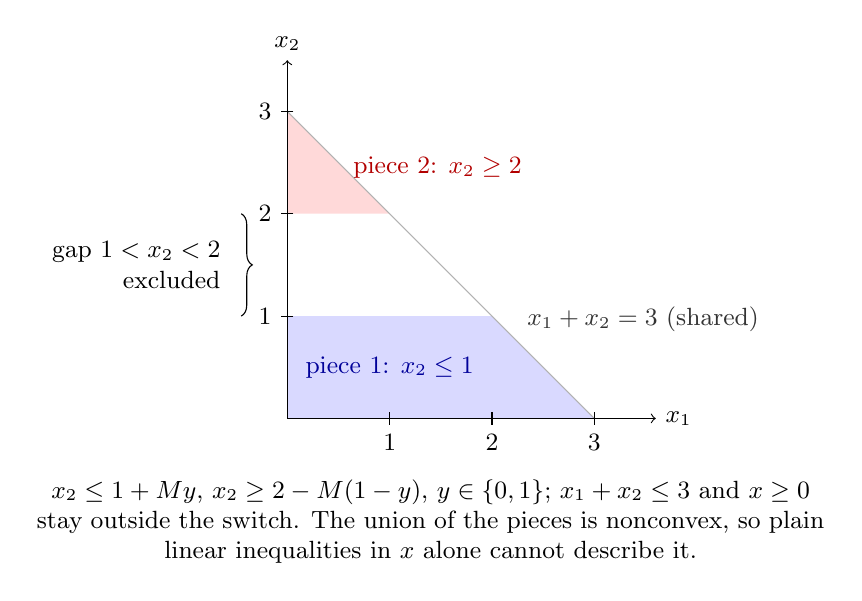
\begin{tikzpicture}[every node/.style={font=\small}, x=1.3cm, y=1.3cm]
	\fill[blue!15] (0,0) -- (3,0) -- (2,1) -- (0,1) -- cycle;
	\fill[red!15] (0,2) -- (1,2) -- (0,3) -- cycle;
	\draw[gray!60] (3,0) -- (0,3) node[pos=0.25, above right, text=gray!40!black] {$x_1+x_2=3$ (shared)};
	\draw[->] (0,0) -- (3.6,0) node[right] {$x_1$};
	\draw[->] (0,0) -- (0,3.5) node[above] {$x_2$};
	\foreach \x in {1,2,3} {\draw (\x,0.06) -- (\x,-0.06) node[below] {$\x$};}
	\foreach \y in {1,2,3} {\draw (0.06,\y) -- (-0.06,\y) node[left] {$\y$};}
	\node[blue!60!black] at (1.0,0.5) {piece 1: $x_2\le1$};
	\node[red!70!black, anchor=west] at (0.55,2.45) {piece 2: $x_2\ge2$};
	\draw[decoration={brace, amplitude=4pt}, decorate] (-0.45,2) -- (-0.45,1) node[midway, left=4pt, align=right] {gap $1<x_2<2$\\ excluded};
	\node[anchor=north, align=flush center, text width=10cm] at (1.4,-0.5) {$x_2\le1+My$, $x_2\ge2-M(1-y)$, $y\in\{0,1\}$; $x_1+x_2\le3$ and $x\ge0$ stay outside the switch. The union of the pieces is nonconvex, so plain linear inequalities in $x$ alone cannot describe it.};
\end{tikzpicture}
\end{document}
